\documentclass[onecolumn]{article}

\usepackage{geometry}
\geometry{textwidth = 18cm,textheight = 24cm}

\usepackage{cite}
\usepackage{caption}
\usepackage{graphicx}
\usepackage{amsmath}
\usepackage{amssymb}
%\usepackage{braket}
\usepackage{textcomp}
%\usepackage{lmodern}
\usepackage{authblk}
\usepackage{datetime}
%\usepackage{gensymb}
\usepackage{wrapfig}
%\usepackage[usenames,dvipsnames,svgnames,table]{xcolor}
%\usepackage{booktabs}
\usepackage{enumitem}
\setlist{nosep}
%\usepackage{appendix}

%\usepackage[switch,columnwise]{lineno}
%\linenumbers

\newcommand{\onlinecite}[1]{\hspace{-1 ex} \nocite{#1}\citenum{#1}} 

\let\OLDthebibliography\thebibliography
\renewcommand\thebibliography[1]{
  \OLDthebibliography{#1}
  \setlength{\parskip}{0pt}
  \setlength{\itemsep}{0pt plus 0.3ex}
}
  
\title{Comparison of semiconducting and superconducting hardware for optoelectronic neuromorphic systems}
\author[1]{\Large{Bryce Primavera and Jeff Shainline}
\\
\textit{\large{National Institute of Standards and Technology}}
\\
\vspace{-0.2em}
\textit{\large{325 Broadway, Boulder, CO, USA, 80305}}
\\
%\vspace{-0.2em}
%\textit{\large{bryce.primavera@nist.gov, jeffrey.shainline@nist.gov}}
}
\date{\today}%\today

\begin{document}

\maketitle
\begin{abstract}
\vspace{3em}
\end{abstract}

%\keywords{neural systems, neuromorphic computing, artificial intelligence, semiconductor devices, superconductor devices}
	
\setcounter{tocdepth}{3}
\setcounter{secnumdepth}{4}
\tableofcontents	
	
\section{\label{sec:introduction}Introduction}
Lay out the problem: 
\begin{itemize}
\item objective: neuromorphic supercomputing, scale of human brain
\item machines that perform cognition
\item not edge
\item not focused on a single metric like speed or power, but rather on overall system scalability and performance
\item seek the highest-performing artificial intelligence
\item system considerations are paramount
\item attempt to find physical limits of cognitive systems
\item device features cannot be introduced if they are highly sensitive or require external tuning
\item present-day neuromorphic cognitive systems using mosfets struggle in communication
\item AER is a great way to make progress with existing hardware, but ultimately becomes a limiting factor
\item optical communication may alleviate bottlenecks simply by avoiding wiring parasitics
\item optical communication may enable the largest neuronal pool \cite{sh2018_ICRC}, which we assume correlates with high cognition
\item we consider here an architecture with a single light source at each neuron
\item this light source emits pulses playing the role of action potentials each time a neuron fires
\item we do not consider any frequency or spatial multiplexing concepts from optical communications here, as they tend to introduce requirements for precise device tolerances or active control of elements that are not scalable to the size of systems we seek
\item action potentials are simply bursts of incoherent photons that a routed to all synaptic connections on a directional branching tree distribution network that taps off equal quantities of light to each synaptic connection
\item photonic action potentials are received as binary communication signals
\item synaptic weights and subsequent processing/computation is performed entirely in the electronic domain; light is used exclusively for communication
\item the new challenge is that integrated light sources do not exist that can be placed at every neuron across a silicon wafer with modern VLSI technology
\item the route to such an integrated device would be far easier if silicon light sources could be employed, an option if one accepts cryogenic operation
\item here we assume such an option will be available at a future date
\item the primary objective of the present study is to compare two approaches to the electronic circuits that would accompany such an optical communication network for large-scale cognitive systems
\item the two approaches are semiconducting circuits and hybrid semiconducting/superconducting circuits
\item in the semi case, photodetectors are waveguide-integrated semiconductor photodiodes, all computational circuits are based on mosfets, and light sources are waveguide-integrated semiconductor leds or lasers (focus on leds for processing/operation simplicity)
\item in the super case, photodetectors are waveguide-integrated snspds, synaptic and dendritic circuits are based primarily on jjs coupled through mutual inductors, neuron circuits combine superconducting and semiconducting components, and the same light sources are employed
\item we attempt to determine which of these approaches to neuromorphic hardware is likely to achieve superior cognitive performance by assessing their functionality in reference to established metrics from neuroscience and cognitive computing
\item we describe these metrics in Sec.\,\ref{sec:neural_device_requirements}.
\item we're not seeking biologically plausible time scales, but rather time scales from as long as possible to as fast as possible, working with the hypothesis that systems that have correlated dynamics and memory over as broad a range as possible will achieve optimal cognition
\end{itemize}

One way this paper could proceed is to compare mosfet-based circuits that implement the relevant operations as described in Ref.\,\cite{chst2014} with soens circuits as discussed in Refs.\,\cite{shbu2019,sh2020}. Reference \cite{chst2014} describes mosfet circuits leveraging subthreshold operation principles to achieve short-term and long-term synaptic plasticity, adaptive threshold, spike production, and scaling to networks. Dendritic processing is not discussed. If we can do an excellent job understanding these circuits and determining how to couple the synaptic receivers to a photodetector and the spike production circuits to a light source, we should have most of what we need to do our comparison. The study could essentially be a comparison of the optoelectronic versions of the circuits in Ref.\,\cite{chst2014} with those in Refs.\,\cite{shbu2019,sh2020}. A lot of the relevant work regarding soens has been done previously, but a few details may need to be considered, such as how the spiking activity of a neuron provides a feedback signal to all of its synapses for plasticity. Additional work may be required on the beyond-stdp learning rules.

Ref.\,\cite{chst2014} discusses hardware/software ecosystem. It appears likely that using photonic communication without AER will lead to significant reduction in complexity of network configuration, potentially significantly reducing the demands on software to control the system. This does come at the cost of reduced reconfigurability of networks.

The circuits in Ref.\,\cite{chst2014} are subthreshold current-mode circuits. Are there any basic physical statements we can make about using photodiodes (which are current-mode circuits) as inputs?

Attention should be paid to device mismatch and tolerances, aspects that affect subthreshold mosfets as well as jjs. Can we determine whether one system will suffer less than the other? Does it matter? Can networks of adaptive, spiking neurons compensate?

MOSFET model: using predictive technology model (PTM) from ASU.

It is not our intention to argue that certain technologies should not be investigated. At this early stage in the development of this complex field, many ideas should be pursued. It is also not clear that in the long-term technological limit, a single, primary technology will dominate. It is possible that many different approaches to adaptive, intelligent, neuromorphic systems will reach maturity and excel in different contexts. Most starkly, one does not expect devices and systems optimized for small-scale, power-starved, edge applications to take the same form as devices and systems optimized for extreme cognitive performance, considering the objectives and constraints are significantly divergent. 

It is our intention instead to assess whether superconducting optoelectronic neural systems deserve to be in the pool of contenders as a hardware platform for achieving extreme cognitive performance. The concept begins from the zeroth order, intuitive (to us) conjectures that 1) optical communication is physically optimal at large scale, 2) few-photon communication is advantageous from a power perspective. First-order elucidation that JJ circuits with diverse circuit parameters, spiking and thresholding behaviors, and convenient activity-based adaptive responses led us to the state of tempered optimism that such hardware might be capable of realizing large-scale spiking neural networks, potentially capable of general intelligence. Yet advocating for hardware combining semiconductors, superconductors, and photonics positions one at the tri-critical point, balanced between compatriot and pariah in all three communities. It is our objective to assess whether the superconducting optoelectronic approach to large-scale neural sytems for artificial intelligence withstands this round of second-order analyses where we subject the concept to scrutiny from numerous angles and quantitatively compare its modeled performance relative to a semiconductor optoelectronic approach that may be more palatable to the community, perhaps by 1/3. Our position would surely be less lonely if we could motivate others to join the soens pursuit, and we hope the study presented here represents prudent analysis that can give us confidence to second order that we are on the right track and can be justified when encouraging others to try playing in this sandbox.

This work is largely motivated by a scientific question, albeit one with potentially significant technological ramifications: is it possible to construct an apparatus as generally intelligent as a human being? Going one step further, what are the physical limits of cognitive intelligence?

\section{Key Takeaway Messages}
\begin{itemize}

\item With light for communication as an assumption, we can converge for both systems to a coarse description that appears feasible:
\begin{itemize}
\item wafer-scale processing
\item multiplanar waveguides across wafers
\item free-space vertical links
\item fluid cooling between wafers
\item fiber-optic white matter over longer distances
\item modular, hierarchical construction over spatial and temporal scales limited by the light cone
\end{itemize}

\item System power required for cryogenic cooling even for a system at rest dictates that superconducting systems will not be more energy efficient than semiconductor systems until a certain scale, roughly the scale at which semiconductor systems dissipate a few hundred watts. This is not edge. It is neuromorphic supercomputing. Crossover is probably around 10$^6$ neurons. Include crossover plot.

\item Assuming area is limited by wgs, need roughly 20 planes of waveguides. This is a necessary demonstration for either platform to be valid.

\item with 20 wg planes of passive waveguides, the situation is significantly improved if photodetectors (diodes or spds) can be integrated with these planes so the synaptic processing can be distributed over the planes instead of residing in a single 2D plane on the substrate. This achieves roughly $20\,\times$ increase in the number of synapses that can be accommodated on a wafer. Multiple planes of waveguides with integrated detectors are a necessary demonstration for poth platforms.

\item In addition to detectors, computational circuits associated with synapses must be spread across multiple planes. Neurons and associated transmitter circuits are far less numerous than synapses, so all neural firing circuits may exist on a single plane, such as the crystalline body silicon of an SOI wafer. But because synapses are far more numerous, and learning/plasticity circuits are not particularly small, electrical circuitry associated with synaptic and dendritic processing must be interspersed with photonic waveguides to fill space in the third dimension above the waver surface. Multiple planes of synaptic circuitry must be demonstrated for both hardware platforms.

\item Power density will be low enough to be removed by water or He at wafer scale, module, up the hierarchy. Volume must be available for grey matter, white matter, and cooling fluid.

\item For semi PD to compete with snspd, receiverless, 200\,aF links are required. This is an element that must be demonstrated.

\item Based on noise considerations on PD at 300\,K, $>\,10^3$ photons are required to be received during a synapse event, as compared to 1 in the spd case. The associated demands on the light source and transmitter driver circuits are correspondingly increased. This means that to fire at the same rate, the semi neuron axon hillock would need to produce roughly 1000$\,\times$ the number of photons as the super case to achieve a snr of 1. By contrast, snspds don't have current or voltage noise in the same sense. (begs further noise analysis (god, it never ends))

\item Regarding light sources, these demands require sources with high efficiency (including coupling and propagation loss) being driven with high current. Demonstration of light sources and driver circuits with sufficient output and wafer scale integration ($10^6 - 10^7$ sources per 300-mm wafer) is a necessary demonstration.

\item These integration requirements sketch the process stack to be pursued in each case
\begin{itemize}
\item semi: one plane mosfets and light sources for transmitters, $N$ superplanes interspersing passive waveguides, poly-si pds, poly-si mosfets for synapses, and mos capacitors for time constants. synaptic  poly-si pds and mosfets require high-temp dopant drive in, so it is unlikely these would be processed after integration with light sources. wafer bonding of synapses and interconnects to neuron transmitter circuits appears likely. potentially an expensive step.
\item super: one plane mosfets and/or hTrons and light sources (potentially silicon, monolithic with mosfets) and $N$ superplanes of passive waveguides, snspds, jjs and inudctors (mutual and kinetic). here, no high temperatures are requried to activate dopants or form ohmic contacts, so these layers could potentially be integrated on wafers with driver circuits and light sources monolithically without the need for wafer bonding. 
\end{itemize}

\item Due to num photons requirements, it is difficult for semi systems to fire much faster than 20\,MHz due to the requirements of the transmitter circuit and light sources to provide photons to all synapses.

\item (aside: what is the total current delivered to each system to drive the light sources?)

\item Memory
\begin{itemize}
\item for semi, floating gate mosfet would be ideal, but has proven difficult. signals necessary to change charge on gate are not the same as the signals typically sent from neurons to synapses. Numerous other devices are being investigated, but a compelling case remains to be made that any of these can rival the adaptation mechanisms supporting learning in the brain. New advances must be made for short-term, long-term, meta, and homeostatic plasticity.
\item for super, plasticity appears straightforward through adaptive flux storage loops coupled to biases of squids in synaptic and dendritic receivers. However, these circuits have only been shown in theory and simulations. experimental demonstrations are necessary. further, the circuits are large, and must be packed densely. it must be demonstrated that this dense, multiplanar packing of coupling circuits through transformers is possible with low cross talk between flux-storage loops.
\end{itemize}

\item in neither the semi or super case is a state-of-the-art technology node required. 45\,nm lithography will suffice for either approach.

\end{itemize}

\vspace{3em}

Summary of demonstrations required of each hardware platform if brain-scale neuromorphic systems are to be feasible.\newline

Necessary semiconductor demonstrations:
\begin{itemize}
\item Wafer-scale integration of $\sim\,20$ planes back-end-of-line passive dielectric photonic waveguides with $\le\,3$\,dB propagation loss from any neuron to any other
\item Integration of multiple planes of photodiodes integrated with low-loss dielectric waveguides (i.e., SiN waveguides evanescently coupled to aSi photodiodes)
\item Integration of multiple planes of mosfets and capacitors performing synaptic computations, plasticity functions, and dendritic processing
\item Receiverless photodetectors with $\mathcal{O}$(200\,aF) capacitance
\item Wafer-scale integration of $10^6$ light sources and driver circuits producing $10^6$ photons within 50\,ns
\item New advances must be made for short-term, long-term, meta, and homeostatic plasticity
\end{itemize}

\vspace{2em}
Necessary superconductor demonstrations:
\begin{itemize}
\item Wafer-scale integration of $\sim\,20$ planes back-end-of-line passive dielectric photonic waveguides with $\le\,3$\,dB propagation loss from any neuron to any other
\item Integration of multiple planes of snspds integrated with low-loss dielectric waveguides (i.e., SiN waveguides evanescently coupled to snspds operating at the correct temperature)
\item Integration of multiple planes of jjs and mutual inductors performing synaptic computations, plasticity functions, and dendritic processing
\item Wafer-scale integration of $10^6$ light sources and driver circuits producing $10^4$ photons within 50\,ns
\item Experimental demonstrations must be made for short-term, long-term, meta, and homeostatic plasticity circuits (multiplanar with low cross talk and sufficiently small area to not dominate total system size)
\end{itemize}



\section{\label{sec:neural_device_requirements}Device requirements for neuromorphic systems}
\begin{itemize}
\item synaptic
\item dendritic
\item neuronal
\item communication network
\end{itemize}
	
\section{\label{sec:light_sources}Light Sources}
Short section, pointing out we're trying to consider systems with similar light sources, hopefully silicon, operated at low temp. Temp could be 77K or 40K or 4K, but we'll try to assume it doesn't matter. 
	
\section{\label{sec:interconnection}Interconnection network and fan-out}
Short section. Similarly to \ref{sec:light_sources}, we want to assume semi and super systems are using the same concepts and hardware for the interconnection network. Fan-out (out degree) is constrained to be the same for the two systems, so light sources and transmitter driver circuits must be scaled to produce the appropriate number of photons.

With such an optical communication scheme, large networks of neurons can be implemented in an asynchronous manner without address requirements that lead to memory challenges in large networks. Each communication channel from a neuron to a synapse has a dedicated waveguide connection, so no time-multiplexing is required. One waveguide leaves each neuron, and it branches as needed to achieve the desired graph structure.

\section{\label{sec:detectors}Detectors}
Important section. 
\begin{itemize}
\item Analyze responsivity and noise to determine how many photons must be incident per pulse on snspd and photodiode to achieve a certain error ($<1\%$, for example)
\item Consider energy consumption of detector per pulse
\item also any quiescent power consumption
\item area
\item fabrication
\item give reasons not to use APDs (Razavi \cite{ra2012}, pg. 57)
\item therefore, not using semiconductor single-photon detectors
\end{itemize}

\vspace{2em}
\noindent Responsivity: $I_p = R_{ph}P_{op}$, where $I_p$ is current generated by photodiode, $R_{ph}$ is the responsivity, and $P_{op}$ is the optical power.

\vspace{2em}
\noindent quantum efficiency: $\eta = \frac{I_p/q}{P_{op}/(hc/\lambda)} = \frac{1.24R_{ph}}{\lambda} = \frac{1}{1+\tau_{r}/\tau_{nr}}$

\vspace{2em}
\noindent Receiver error rate: is Razavi's noise/error rate model correct for us? We need to pay special attention to two limiting cases: 1) a single spike is received after a long period of rest (string of zeros); and 2) a fast spike train is received (burst input) (one zero one zero ...) Compare Razavi's analysis to Bryce's calculation. 

Here's Bryce's calculation:

\subsection{Motivation}
The ultimate goal of this project will be to compare the performance and feasibility of various incoherent optoelectronic platforms for neuromorphic computing. Semiconductor photodetectors have already become a ubiquitous technology and are consequently a natural starting point for a whole class of potential optoelectronic neuromorphic hardware. This short summary seeks to accomplish two goals: (1) To determine the minimum optical power required for the detector to register an optical spiking event and (2) to analyze both the static and dynamic energy dissipation in a detector.

\subsection{Photodetector Basics and Noise}
%\quad DERIVATION PRIMARILY DRAWN FROM THESE TWO SOURCES:
%\newline
%\hyperlink{http://ecee.colorado.edu/~bart/ecen6355/chapt-05.pdf}{http://ecee.colorado.edu/~bart/ecen6355/chapt-05.pdf} - section 5.1.2 pages 5.9-5.11
%\newline
%\hyperlink{https://users.physics.ox.ac.uk/~rtaylor/teaching/Opto_lecture5.pdf}{https://users.physics.ox.ac.uk/~rtaylor/teaching/Opto_lecture5.pdf} - section 4, pages 7-9
%\newline

The most basic parameter for a photodetector is the \textit{responsivity}, $\mathcal{R}$. The responsivity is simply the ratio of photocurrent to input optical power. It is related to the external efficiency, $\eta$ as shown below:
\begin{equation}
    \mathcal{R} = \frac{q\eta\lambda}{hc}
\end{equation}
where $\lambda$ is the wavelength of the incoming light. $\eta$, and therefore $\mathcal{R}$, can be expected to be strong functions of wavelength. With responsivity defined, it is straightforward to predict the amount of photocurrent ($I_{ph}$) produced for a certain input optical power ($P_{opt}$):
\begin{equation}
    I_{ph} = \mathcal{R}P_{opt}
\end{equation}

In order to produce a measurable response, the photocurrent must be larger than the RMS fluctuations of the noise current. There are two primary sources of this noise in photodiodes - dark current noise and Johnson Noise from the load resistor. The noise from the dark current will be considered first. The RMS fluctuations can be given as:
\begin{equation}
    <I^{2}> = 2qI\Delta f
\end{equation}
$I$ is simply the total current flowing through the diode and $\Delta f$ is the bandwidth of the detector. This is already an interesting detail, as the noise can potentially be reduced by operating at a lower bandwidth (I guess this corresponds to something like integrating the signal?). For this paper, I will take the bandwidth to be 20 MHz, for sake of comparison with SOENS. In principle all sources of current - ideal diode current, SHR, band-to-band recombination, and photocurrent - should be included in $I$. 

We can approximate $I = I_{D} + I_{ph}$, where $I_{D}$ is the dark current. There is an additional Johnson Noise associated with the load resistor, $R_{L}$. This leads to a total noise, $I_{N}$ of:
\begin{equation}
    I_{N} = \sqrt{2qI\Delta f + \frac{4k_{B}T\Delta f}{R_{L}}}
\end{equation}
Equating the photocurrent with the RMS noise fluctuations gives an estimate of the bare minimum detectable optical power.
\begin{equation}
    P_{min} = \frac{I_N}{\mathcal{R}}
\end{equation}
Or in terms of the minimum necessary photocurrent, $I_{ph}$:
\begin{equation}
    I_{ph} = \sqrt{2q(I_D+I_{ph})\Delta f + \frac{4k_{B}T\Delta f}{R_{L}}
    }
\end{equation}

Solving the quadratic equation for $I_{ph}$ yields:
\begin{equation}
    I_{ph} = q\Delta f(1+\sqrt{1+\frac{2I_D+}{q\Delta f} +
    \frac{4k_BT}{q^2R_L\Delta f}})
\end{equation}
where $I_R = \sqrt{\frac{4k_{B}T\Delta f}{R_{L}}}$, the contribution to the noise current from the Johnson noise of the resistor. The minimum optical power, $P_{min}$ follows from the responsivity:
\begin{equation}
    P_{min} = \frac{I_{ph}}{\mathcal{R}}=
    \frac{q\Delta f}{\mathcal{R}}(1+\sqrt{1+\frac{2I_D}{q\Delta f} +
    \frac{4k_BT}{q^2R_L\Delta f}})
\end{equation}

The next task is to determine the appropriate temporal length of an optical spike. For a photodetector operating at its maximum rate, it suffices to use 1/$\Delta f$ as the duration of spike. Of course, this duration will likely be set by the speed of the LED, but for now I'm going to just assume that the bandwidth of our receiver circuit was designed to coincide with the bandwidth of the LED. In this case, with photon energy $E_{ph}$, the necessary number of photons per spike ($N$) is then:
\begin{equation}
    N = \frac{P_{min}}{E_{ph}\Delta f}
\end{equation}

A plot of the minimum number of photons per spike vs bandwidth is presented in Figure 1. From experimenting with some plausible parameters, it seems likely that noise will be dominated by the Johnson Noise in the load resistor. This noise can be reduced by utilizing a larger resistor. However, a larger $R_L$ will degrade the bandwidth of the circuit. A lower bandwidth requires the light source to be on for longer and increases the necessary optical power. In Figure 1, the color-coded vertical lines represent the maximum frequency that a 10pF photodiode could respond at. In fact, since the bandwidth is inversely proportional to $R_L$, it can be seen from equation 8 that in the resistor dominated noise regime, N will become independent of $R_L$. Fortunately, this bandwidth limit can be beaten by using a transimpedance amplifier as we will see in following sections.
\begin{figure}
    \centering
    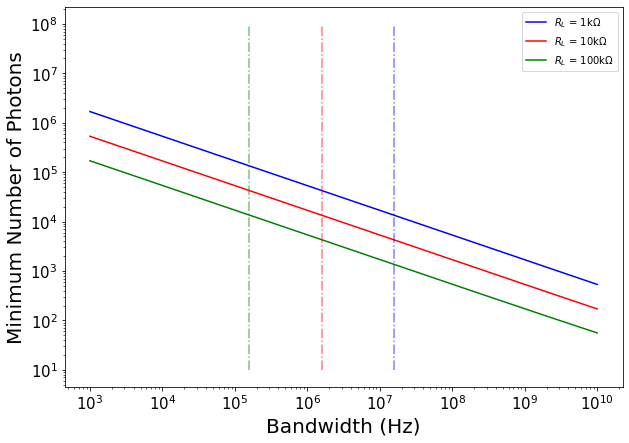
\includegraphics[width=8.6cm]{photon_V_BW.png}
    \caption{A plot of the minimum number of photons needed per spike as a function of Bandwidth. $I_D$ = 10nA, $\mathcal{R}$ = .5, and $\lambda$ = 1.3$\mu$m. The dotted vertical lines correspond to the maximum frequency achievable without a transimpedance amplifier for a 10pF photodiode. }
    \label{fig:my_label}
\end{figure}

Finally, we can also see a simple example of explicit temperature dependence. $I_D$ is a strong function of temperature and will play a role when we get to static power dissipation, but the Johnson noise in the resistors is more important for determining the minimum optical signal. It has a simple square root temperature dependence, which can be seen in figure 2.
\begin{figure}
    \centering
    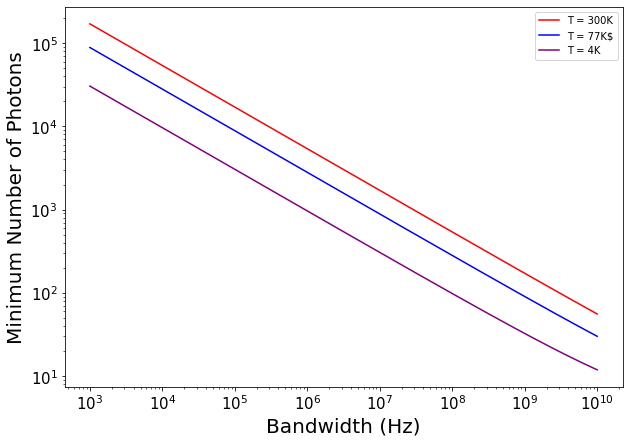
\includegraphics[width=8.6cm]{Temp_Photon_spike.png}
    \caption{Temperature dependence of the minimum optical signal. $R_L = 100k\Omega$}
    \label{fig:my_label}
\end{figure}

\subsection{Transimpedance amplifier}

\section{\label{sec:synapses}Synaptic circuits and weighting}
Important section.
\begin{itemize}
\item comparison of possible functionalities
\begin{itemize}
\item short-term facilitating
\item short-term depressing
\item long-term event-based potentiation/depression (STDP)
\end{itemize}
\item for each, consider information-processing metrics such as range of operation, bit depth 
\item for each, also consider area, power
\item also sensitivity (exponential weight dependence on voltage in subthreshold mosfet vs polynomial (almost linear) weight dependence on current in soens)
\item discuss in the context of Fusi's work (\cite{amfu1994,fudr2005,fuab2007})
\item it may just be that semiconductor-compatible approaches to memory appear weaker because they have had more time to be scrutinized
\end{itemize}

\section{\label{sec:dendrites}Dendrites and fan-in}

\section{\label{sec:neurons}Neural integration and threshold}

\section{\label{sec:adaptation}Synaptic, dendritic, and neuronal adaptation}
Discuss options for short- and long-term synaptic plasticity;, adaptive dendritic functions; and neuronal refractory period, spike-frequency adaptation, and homeostatic plasticity (threshold adaptation).

\subsection{Memristors}

\begin{itemize}

\item Synaptic adaptation occurs due to atomic motion within the material. This means all time constants and signal levels necessary for adaptation are strongly coupled to material parameters. Rather than designing a circuit with essentially arbitrary time constants and signal levels that are exactly the same as the signal levels used elsewhere in the system for information processing, one must explore many materials and find the ones that work closest to the signal levels used for the rest of dendritic and neuronal processing.

\item Motion at the atomic level also risks degradation over time. If such a synapse performs short-term adaptation (with conductance changing on the time scale of the inter-spike interval), even materials that can survive billions of cycles will reach the end of life in a matter of days, assuming synapses receive inputs on average at 1\,kHz, as expected for optoelectronic neurons

\item One may argue synaptic plasticity occurs due to structural changes at the nanoscale (particularly long-term adaptation), so memristor mechanisms are similar to biology in this regard. However, the assembly of molecular machines at the nanoscale via protein synthesis and construction leads to the potential for growth and regeneration in a manner that will be difficult for memristors to match. Memristors will suffer from the second law of thermodynamics, eventually succumbing to a homogeneous, disordered state, while the organizing capabilities of biological synapses locally circumvent this inconvenient propensity.

\item The plasticity mechanisms proposed in soens are based around achieving desired functionality through circuit design, with complexity and responses limited primarily by area, while the plasticity mechanisms leveraged in memristors are based on material properties, and are therefore limited primarily by the physics of the universe. There is a large parameter space to explore in both cases, but circuit design provides much more opportunity for flexibility and implementation of diverse responses across the network, while diverse responses from memristors may require a large number of different materials, which will be difficult to fabricate for practical reasons.

\item The strength of memristors is exactly the weakness of soens: memristors can be made very small.

\item It may be helpful to have metaplastic neuromodulatory control, so a region of synapses can adapt more or less rapidly at various times. With the circuit approach this can be accomplished by varying common current or voltage biases. Is there an analogous mechanism for memristors? Can you change their rate of adaptation collectively, not based on their individual history of activity, but by other mechanisms based on network activity across larger regions?

\item What is stdp time constant in the brain?

\item memristors are often used in crossbar arrays, usually in feed-forward architectures. we need a plausible circuit design for how we would use it to set synaptic weight.

\end{itemize}

\section{\label{sec:transmitters}Transmitter driver circuits}

\section{\label{sec:time_constants}Time constants and subthreshold oscillations}

\section{\label{sec:biasing}Biasing}

\section{\label{sec:systems}Power consumption, cooling, and system considerations (including fabrication and production)}

%\begin{figure}[tb]
%    \centering{\includegraphics[width=8.6cm]{superconducting_gap.pdf}}
%	\captionof{figure}{\label{fig:superconducting_gap}Approximate normalized superconducting energy gap of niobium as a function of temperature.}
%\end{figure}

%\begin{equation}
%\label{eq:energy_gap}
%\frac{\Delta(T)}{\Delta(0)} \sim \bigg[1-\bigg(\frac{T}{T_c}\bigg)^{3.3}\bigg]^{1/2},
%\end{equation}

\section{Notes}
Differences between neural and digital optical communication:
\begin{itemize}
\item neural: mux/demux not required
\item neural: high power optical signals not necessary (nor tolerable)
\item neural: not point to point, one to many
\item neural: asynchronous, no clock, no phase-locked loop, no clock recovery on receive
\item neural: 1s and 0s not equally common; signals are sparse
\item neural: TIA + limiting amplifier + decision circuit likely uses too much power
\item neural: noise is more tolerable, decision circuit still potentially useful
\item neural: speed can be much lower, as demonstrated by biology
\item neural: with lower light levels, light-source driver circuits don't need to deliver as much current
\item multi-chip partitioning required for digital due to high speed and sensitivity to timing jitter, multi-chip not tolerable for neural (cannot have multiple chips for each neuron) Tx and Rx amplifiers cannot remain in isolation (\cite{ra2012} pg. 5)
\item neural: bits are not sampled on a clock
\end{itemize}

other notes:
\begin{itemize}
\item in conventional optical communication systems, package parasitics limit speed. optoelectronic integration crucial for overcoming this limitation (\cite{ra2012} pg. 5)
\item for long time constants, semiconductors can augment RC by op amp gain: $RC \rightarrow (1+A)RC$, where $A$ is the op amp gain, which can be enormous, like 300,000. thus, essentially arbitrarily long time constants can be achieved. the price is power.
\item regarding subthreshold oscillations, RLC behavior in semiconductors can be achieved with op amps. in this case, there is no inductor, and that role is played by the active op amp. the price is power
\end{itemize}

\section{Acknowledgements}

\vspace{1em}
\noindent This is a contribution of NIST, an agency of the US government, not subject to copyright.

%\clearpage
%\newpage
\appendix
%\appendixpage

\section{\label{apx:one}Appendix One}
Appendix One

\bibliographystyle{unsrt}	
\bibliography{ss_comparison}

\end{document}